
\section{Решения письменных задач.}

В уровне 2 также есть письменная задача, которую нужно сдавать в письменном виде. Целесообразно после того, как все сдадут письменные задачи обоих уровней (или большинство, если все-таки  есть те, кому через значительное время не удалось получить второй уровень), выдать письменные решения. 



\textbf{Задача \ref{1.4}}$^n$ Может ли для каких-нибудь целых чисел $a$ и $b$ быть верно:    $$ab(a-b) = 201720182019$$

\begin{prf}
	\textbf{1 способ.} Рассмотрим два случая. 1 случай: числа $a$ и $b$ одной четности. Тогда $a - b$ обязательно четно. Следовательно, произведение $ab(a-b)$ также будет четным. 2 случай: числа a и b разной четности. Тогда в произведении $ab(a-b)$ один из множителей четен и, следовательно, все произведение четно. Тем самым мы доказали, что для любых целых чисел $ а $ и $ b $ произведение $ab(a-b)$ четно. Но число $ 201720182019 $ нечетно, следовательно, требуемое в условии невозможно.
	
	\textbf{2 способ.} Поскольку $ 201720182019 $ -- нечетное число, то требуется выяснить, можно ли его разложить на три нечетных множителя указанного в условии вида. Предположим, что это возможно, тогда числа $a$ и $b$ должны быть нечетными, но тогда $a - b$ обязательно четно. Следовательно, произведение $ab(a-b)$ также будет четным. Противоречие. Следовательно, требуемое в условии невозможно.
\end{prf}

\textbf{Задача \ref{1.21}}$^n$
	В разные моменты времени из пунктов А и В выехали навстречу друг другу велосипедист и мотоциклист. Встретившись в точке С, они тотчас развернулись и поехали обратно. Доехав до своих пунктов, они опять развернулись и поехали навстречу друг другу. На этот раз они встретились в точке D и, развернувшись, вновь поехали к своим пунктам. И т.д. В какой точке отрезка АВ произойдет их 2019 встреча?

\begin{prf}
	В точке С. 
	Без ограничения общности можно считать, что первым выехал кто-то из А. Тогда пусть К - точка, в которой находится этот кто-то в тот момент времени, когда второй выехал из В. Теперь они одновременно стартуют - один из В, другой из К и через некоторое время прибывают в С. С этого момента точка К больше не имеет значения. Они разворачиваются и через некоторое время Т одновременно прибывают в D. И так далее. Заметим, что за время Т вместе оба путешественника проедут удвоенный путь от А до В. (см.рис.). Теперь, если они развернутся в точке D и поедут обратно, то за время Т они снова приедут в точку С (это будет их третья встреча). И так далее. Отсюда следует, что все нечетные встречи будут происходить в точке С, а все четные - в точке D. Поскольку 2019 - нечетное число, то 2019-я встреча состоится в точке С.
\end{prf}

\begin{figure}[h!]
\begin{minipage}{0.69\linewidth}\setlength{\parindent}{1.5em}
\textit{Замечание.} Отметим, что мы не использовали информацию о том, кто именно выехал из какого пункта и какая именно скорость была у путешественников. Используется только неизменность скоростей. Для решения задачи это неважно. Более того, при определенных условиях точки С и D могут совпадать, но это тоже не имеет значения, поскольку приведенные выше рассуждения справедливы и для этого случая.
\end{minipage}
\hfill 
\begin{minipage}{0.3\linewidth}\setlength{\parindent}{1.5em}
    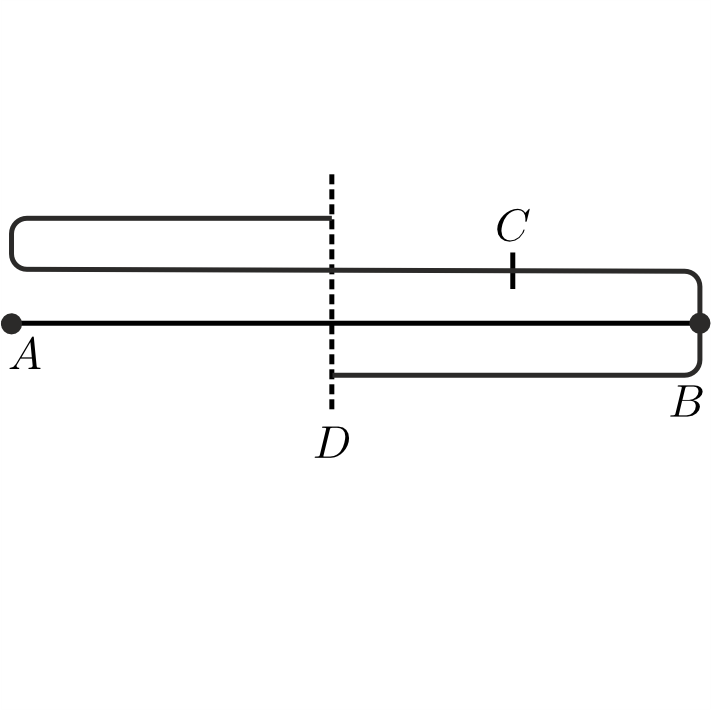
\includegraphics[scale=0.7]{./img/ABC}
\end{minipage}
\end{figure}